%|//////////////////////////////////////|\\\\\\\\\\\\\\\\\\\\\\\\\\\\\\\\\\\\\|%
%|//////////////////////////| Objetivo del Proyecto |\\\\\\\\\\\\\\\\\\\\\\\\\|%
%|//////////////////////////////////////|\\\\\\\\\\\\\\\\\\\\\\\\\\\\\\\\\\\\\|%
\section{Objetivo del Proyecto}
% El objetivo es la respuesta a la pregunta “¿para qué?”; tiene que satisfacer alguna necesidad del usuario.

El presente proyecto consiste en el diseño y desarrollo de un sistema de calibración de impedancia y ajuste por electrodeposición (galvanoplastía). Este instrumento se utilizará en el futuro en aplicaciones biomédicas, más precisamente en la fabricación de electrodos de registro extracelular.



%|//////////////////////////////////////|\\\\\\\\\\\\\\\\\\\\\\\\\\\\\\\\\\\\\|%
%|////////////////////////| Descripción del Proyecto |\\\\\\\\\\\\\\\\\\\\\\\\|%
%|//////////////////////////////////////|\\\\\\\\\\\\\\\\\\\\\\\\\\\\\\\\\\\\\|%
\section{Descripción del Proyecto}
% En esta sección se responde la pregunta “¿cómo?”. Aquí se enumeran las prestaciones, las funciones y el comportamiento o uso del equipo.

El equipo incluye una cuba conductora, que contiene una solución acuosa, donde se colocan los electrodos. Éstos son similares a un filamento de cobre recubierto con esmalte aislante en su totalidad, excepto en los extremos, los cuales uno va sumergido en la solución y el otro conectado al equipo por medio de un conector especial.\\

El sistema funciona con 1, 4, 8, 12 ó 16 electrodos, corrigiendo de a uno por vez. El usuario coloca los electrodos procurando que no se produzcan cortocircuitos entre los mismos (se prevé detectar esto antes de comenzar), selecciona la impedancia final deseada y da la orden de inicio. Luego de algunos chequeos básicos se da comienzo al proceso mostrando un mensaje de inicio. Al terminar con todos los electrodos, se muestra la impedancia final de cada uno. 

En líneas generales, el sistema consta de un primer módulo que consiste en una fuente de corriente alterna (se espera construirla con un amplificador de trasconductancia $i_o/v_i$, utilizando como entrada una señal senoidal de tensión generada en el microcontrolador, obteniendo en la salida una señal de corriente) que se emplea para medir la impedancia de cada electrodo a estudiar. La señal de salida de este circuito es una corriente senoidal de unos \SI{30}{\nano\ampere} y \SI{1}{\kilo\hertz}. Considerando la ley de Ohm y midiendo el valor pico de tensión, se calcula la impedancia del electrodo en estudio como $Z@\SI{1}{\kilo\hertz} = \frac{\hat{v}}{\hat{\i}}$. Luego, un segundo módulo se encarga de imponer una corriente continua de referencia en el sistema, también con un valor de \SI{30}{\nano\ampere} o bien de \SI{120}{\nano\ampere}, para poder disminuir el valor de la impedancia en caso de ser necesario. Esto es posible porque la solución acuosa contiene oro o plata, de modo de que se produce un recubrimiento por \emph{galvanoplastía} sobre el electrodo y así disminuye la impedancia. Si este proceso es necesario o no, dependerá del resultado previo y de la comparación entre el valor obtenido en la medición y el de referencia establecido previamente por el usuario. Estos dos circuitos se conectan mediante multiplexores analógicos (ver diagrama en bloques) que permiten seleccionar la opción correcta de acuerdo a la cantidad de electrodos analizados. 

Como se mencionó, previo a la medición hay que verificar que ningún electrodo esté en cortocircuito con otro. Para ello se propuso inyectar señal en cada electrodo chequeando sobre cada uno de los restantes que no se reciba un nivel elevado de la misma, siendo necesario un multiplexor más, en paralelo con el que se utiliza para inyectar las señales.

Cada determinado tiempo (del orden de \SI{1}{\minute}) tiene que medirse la impedancia y corregirla de ser necesario del modo explicado. Este proceso debe repetirse tantas veces como sea necesario hasta llegar al valor de impedancia deseada determinado previamente en la configuración (los valores aceptables para empezar el proceso están entre \SI{1}{\mega\ohm} y \SI{5}{\mega\ohm}), junto con la cantidad de electrodos utilizados. Además, hay que pautar un tiempo máximo de sensado y corrección, para que el sistema deje de actuar en caso de haber pasado ese tiempo sin haber llegado al valor buscado.



%|//////////////////////////////////////|\\\\\\\\\\\\\\\\\\\\\\\\\\\\\\\\\\\\\|%
%|///////////////| Características y Especificaciones Mínimas |\\\\\\\\\\\\\\\|%
%|//////////////////////////////////////|\\\\\\\\\\\\\\\\\\\\\\\\\\\\\\\\\\\\\|%
\section{Características y Especificaciones Mínimas}
% Las especificaciones acotan las bondades del equipo. Deben listarse los rangos de funcionamiento o requerimientos externos (por ejemplo: tensión de alimentación, consumo, temperatura de funcionamiento, protocolos de comunicaciones, rangos de medición, etc.)

Se presentan las siguientes especificaciones a cumplir:

\begin{table}[H]
\begin{center}
\begin{tabular}{|r|l|}
    \hline
    Tensión de alimentación &
    \SI{5}{\volt} \\ \hline
    Consumo &
    $<$ \SI{500}{\milli\ampere} (\SI{2.5}{\watt}) \\ \hline
    Temperatura de funcionamiento &
    \SI{5}{\celsius} - \SI{70}{\celsius} \\ \hline
    Rango de impedancias de los electrodos medidos &
    \SI{0}{\mega\ohm} - \SI{20}{\mega\ohm} (@ \SI{1}{\kilo\hertz})\\ \hline
    Impedancia buscada & $\simeq$ \SI{1}{\mega\ohm}\\ \hline
    Cantidad de electrodos a conectar &
    1, 4, 8, 12 ó 16 \\ \hline
    Tiempo máximo de corrección por electrodo &
    \SI{60}{\minute} (*)\\ \hline
    Modo medición & señal senoidal, \SI{1}{\kilo\hertz}, error $<$ 10 \% \\ \hline
    Modo corrección & señal continua \SI{30/120}{\nano\ampere}, error $<$ 20\% \\ \hline
\end{tabular}
\end{center}
\end{table}

(*) una vez cumplido este tiempo se abandonan los esfuerzos.


%|//////////////////////////////////////|\\\\\\\\\\\\\\\\\\\\\\\\\\\\\\\\\\\\\|%
%|/////////////////////////| Periféricos Principales |\\\\\\\\\\\\\\\\\\\\\\\\|%
%|//////////////////////////////////////|\\\\\\\\\\\\\\\\\\\\\\\\\\\\\\\\\\\\\|%
\section{Periféricos Principales}
% Los periféricos son los elementos ajenos al microcontrolador con los que interactúa el equipo y deben estar claramente definidos (por ejemplo: motores, display, teclado, puertos de comunicación, sensores, etc.)

El dispositivo tiene una pantalla LCD donde se muestran las opciones de configuración para seleccionar a través de un menú y también los resultados del proceso, además de los mensajes de error o alerta (en caso de ocurrir algún imprevisto o no llegar al valor deseado en el tiempo pautado, por ejemplo). Las opciones se seleccionan desde un teclado de 4 ó [6] botones (\texttt{ok}, \texttt{cancelar}, [\texttt{mover arriba}], [\texttt{mover abajo}], \texttt{mover izquierda}, \texttt{mover derecha}).

Además, como periféricos principales están los dos circuitos mencionados antes, el de medición y el de corrección, a través de los cuales se interactúa directamente con los electrodos. Asimismo, otros elementos importantes con los que interactúa el microcontrolador son los multiplexores, que tienen 1 ó 4 entradas de control, según sean de 2 canales o 16, y la cuba electrolítica donde se produce la reacción química para disminuir la impedancia, que está compuesta por un material conductor, el cual también debe conectarse.



%|//////////////////////////////////////|\\\\\\\\\\\\\\\\\\\\\\\\\\\\\\\\\\\\\|%
%|////////////////| Diagrama en Bloques Preliminar (hardware) |\\\\\\\\\\\\\\\|%
%|//////////////////////////////////////|\\\\\\\\\\\\\\\\\\\\\\\\\\\\\\\\\\\\\|%
\section{Diagrama en Bloques Preliminar (hardware)}
% El esquema general de interconexión de todos los dispositivos importantes se representa mediante un diagrama en bloques.
\begin{center}
    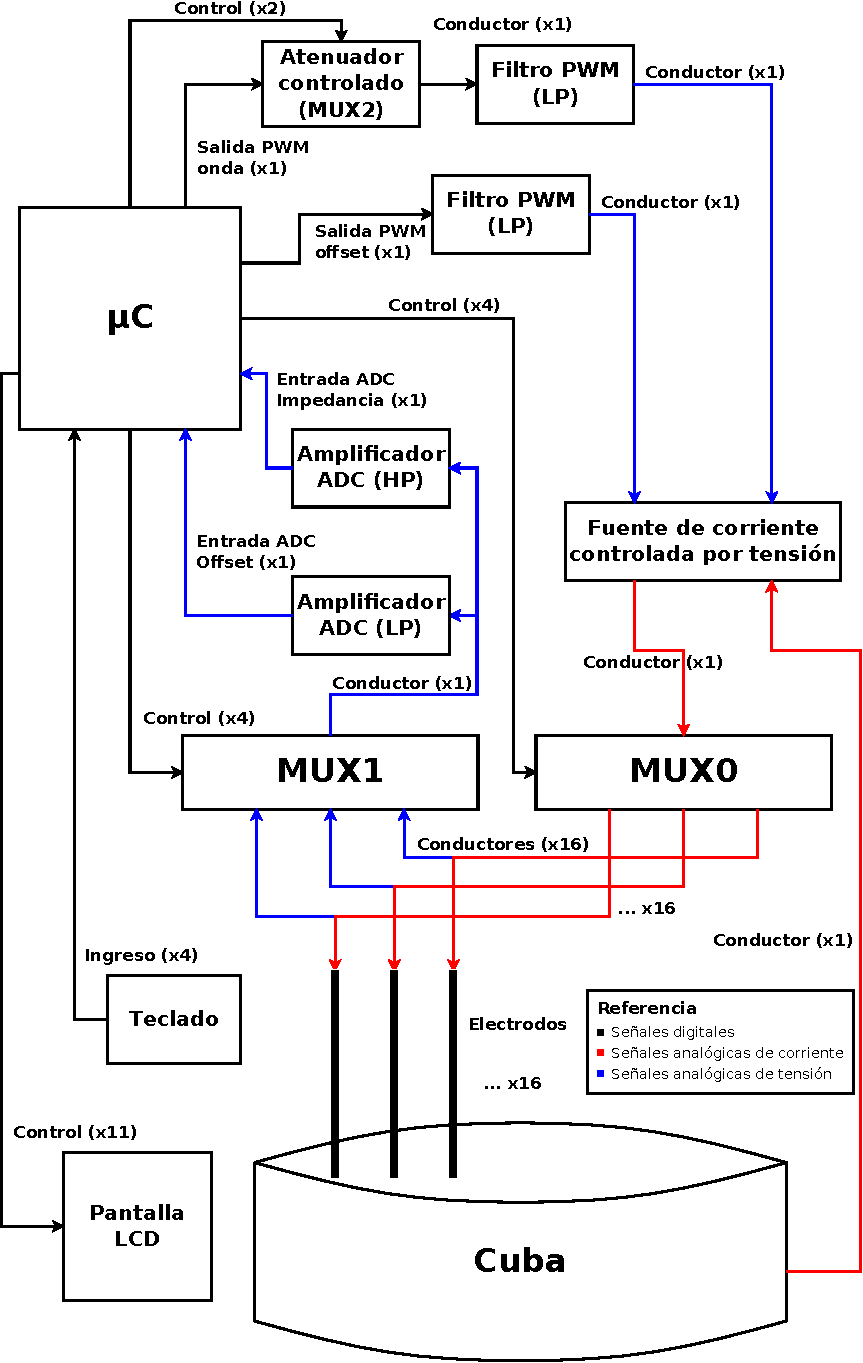
\includegraphics[scale=0.9]{bloques}
\end{center}



%|//////////////////////////////////////|\\\\\\\\\\\\\\\\\\\\\\\\\\\\\\\\\\\\\|%
%|/////////////////| Diagrama de Flujo Preliminar (firmware) |\\\\\\\\\\\\\\\\|%
%|//////////////////////////////////////|\\\\\\\\\\\\\\\\\\\\\\\\\\\\\\\\\\\\\|%
\section{Diagrama de Flujo Preliminar (firmware)}
% El diagrama de flujo ilustra de manera general la interacción entre los distintos bloques (o rutinas) de código.
\begin{center}
    \vspace{-4mm}
    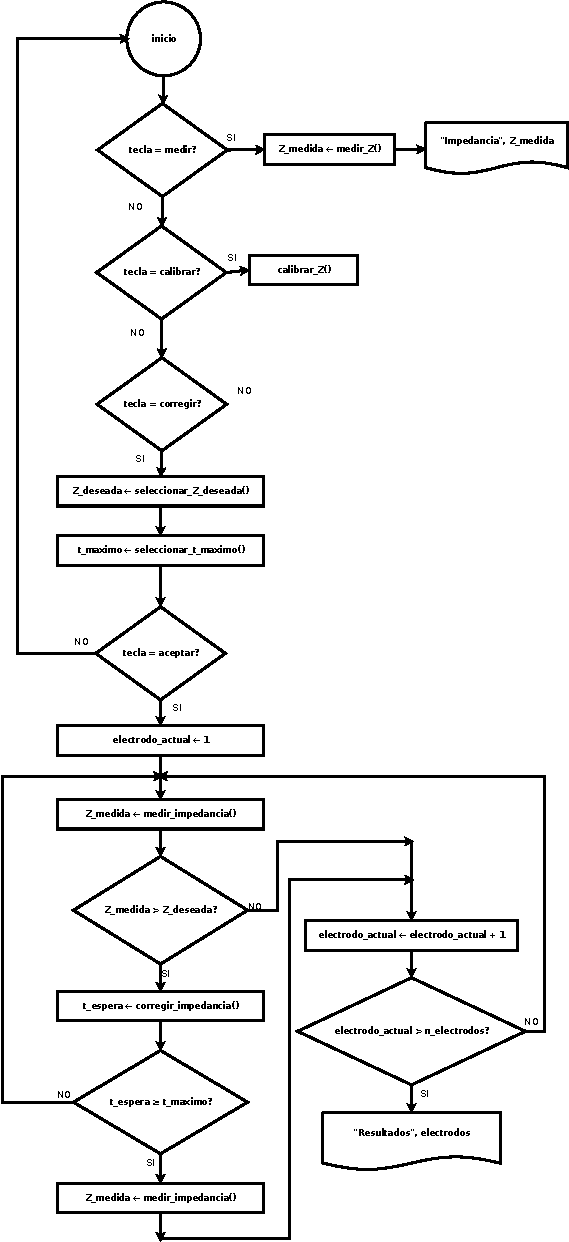
\includegraphics[scale=1.18]{flujo}
\end{center}



%|//////////////////////////////////////|\\\\\\\\\\\\\\\\\\\\\\\\\\\\\\\\\\\\\|%
%|/////////////////////////| Plan de Trabajo (Gantt) |\\\\\\\\\\\\\\\\\\\\\\\\|%
%|//////////////////////////////////////|\\\\\\\\\\\\\\\\\\\\\\\\\\\\\\\\\\\\\|%
\section{Plan de Trabajo (Gantt)}
% Un diagrama de Gantt es la propuesta de distribución de tiempos y recursos a lo largo del proyecto. Es necesario elaborar un plan inicial y ajustarlo en forma continua para no perder de vista el objetivo final, los hitos y el camino crítico para alcanzarlo.
\begin{center}
    \vspace{-4mm}
    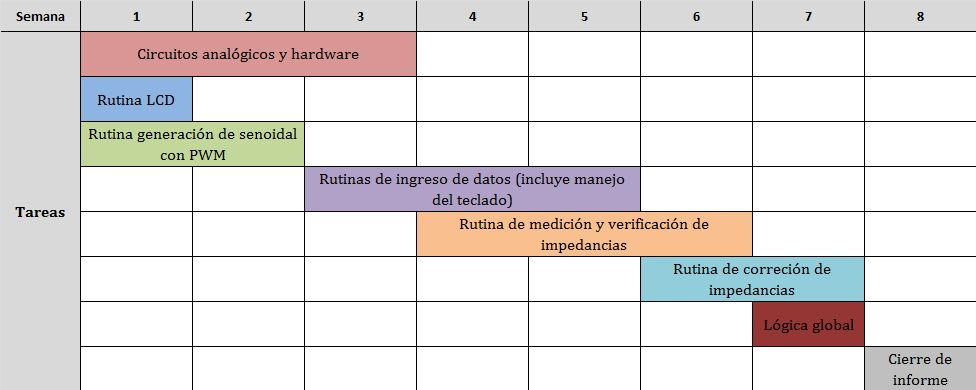
\includegraphics[scale=0.65]{Gantt}
\end{center}


%|//////////////////////////////////////|\\\\\\\\\\\\\\\\\\\\\\\\\\\\\\\\\\\\\|%
%|////////////////| Listado de Componentes y Costos Estimados |\\\\\\\\\\\\\\\|%
%|//////////////////////////////////////|\\\\\\\\\\\\\\\\\\\\\\\\\\\\\\\\\\\\\|%
\section{Listado de Componentes y Costos Estimados}
% En esta instancia se pretende un listado de los componentes más significativos con sus costos aproximados más una previsión general de elementos menores. Lo que se busca es considerar la viabilidad económica del proyecto.
Los componentes más significativos que se emplearán para la construcción del dispositivo se muestran en la tabla siguiente:

\begin{table}[H]
\begin{center}
\begin{tabular}{|r|l|}
    \hline
    \textbf{Componente} &
    \textbf{Costo aproximado} \\ \hline
    Atmega32 & $??$ \\ \hline
    REF200 & $??$ \\ \hline
    OPA128 & $??$ \\ \hline
    INA105 & $??$ \\ \hline
    CD74HC4067 x3 & $??$ \\ \hline
    Resistencias & $??$ \\ \hline
    Capacitores & $??$ \\ \hline
    Display LCD & $??$ \\ \hline
    Pulsadores x6 & $??$ \\ \hline
\end{tabular}
\end{center}
\end{table}

%|//////////////////////////////////////|\\\\\\\\\\\\\\\\\\\\\\\\\\\\\\\\\\\\\|%
%|///////////////////////| Factores Críticos de Éxito |\\\\\\\\\\\\\\\\\\\\\\\|%
%|//////////////////////////////////////|\\\\\\\\\\\\\\\\\\\\\\\\\\\\\\\\\\\\\|%
\section{Factores Críticos de Éxito}
% Es importante analizar cuáles son los riesgos potenciales más importantes que podrían dificultar la realización del proyecto. Una vez identificados, conviene hacerles un seguimiento cercano para evitar contratiempos.
Como factores riesgosos a la hora de cumplir con los objetivos se pueden mencionar:
\begin{itemize}
\item La complejidad de los circuitos analógicos involucrados
\item La resolución a nivel software de la entrada de teclado
\item La generación de la señal seniodal con PWM
\item La coordinación con el IIBM
\end{itemize}